% Options for packages loaded elsewhere
% Options for packages loaded elsewhere
\PassOptionsToPackage{unicode}{hyperref}
\PassOptionsToPackage{hyphens}{url}
\PassOptionsToPackage{dvipsnames,svgnames,x11names}{xcolor}
%
\documentclass[
  10pt,
  letterpaper,
  DIV=11,
  numbers=noendperiod,
  oneside]{scrartcl}
\usepackage{xcolor}
\usepackage[left=1in,marginparwidth=2.0666666666667in,textwidth=4.1333333333333in,marginparsep=0.3in]{geometry}
\usepackage{amsmath,amssymb}
\setcounter{secnumdepth}{-\maxdimen} % remove section numbering
\usepackage{iftex}
\ifPDFTeX
  \usepackage[T1]{fontenc}
  \usepackage[utf8]{inputenc}
  \usepackage{textcomp} % provide euro and other symbols
\else % if luatex or xetex
  \usepackage{unicode-math} % this also loads fontspec
  \defaultfontfeatures{Scale=MatchLowercase}
  \defaultfontfeatures[\rmfamily]{Ligatures=TeX,Scale=1}
\fi
\usepackage{lmodern}
\ifPDFTeX\else
  % xetex/luatex font selection
  \setmainfont[]{TeX Gyre Pagella}
  \setmonofont[]{Fira Code}
  \setmathfont[]{TeX Gyre Pagella Math}
\fi
% Use upquote if available, for straight quotes in verbatim environments
\IfFileExists{upquote.sty}{\usepackage{upquote}}{}
\IfFileExists{microtype.sty}{% use microtype if available
  \usepackage[]{microtype}
  \UseMicrotypeSet[protrusion]{basicmath} % disable protrusion for tt fonts
}{}
\usepackage{setspace}
\makeatletter
\@ifundefined{KOMAClassName}{% if non-KOMA class
  \IfFileExists{parskip.sty}{%
    \usepackage{parskip}
  }{% else
    \setlength{\parindent}{0pt}
    \setlength{\parskip}{6pt plus 2pt minus 1pt}}
}{% if KOMA class
  \KOMAoptions{parskip=half}}
\makeatother
% Make \paragraph and \subparagraph free-standing
\makeatletter
\ifx\paragraph\undefined\else
  \let\oldparagraph\paragraph
  \renewcommand{\paragraph}{
    \@ifstar
      \xxxParagraphStar
      \xxxParagraphNoStar
  }
  \newcommand{\xxxParagraphStar}[1]{\oldparagraph*{#1}\mbox{}}
  \newcommand{\xxxParagraphNoStar}[1]{\oldparagraph{#1}\mbox{}}
\fi
\ifx\subparagraph\undefined\else
  \let\oldsubparagraph\subparagraph
  \renewcommand{\subparagraph}{
    \@ifstar
      \xxxSubParagraphStar
      \xxxSubParagraphNoStar
  }
  \newcommand{\xxxSubParagraphStar}[1]{\oldsubparagraph*{#1}\mbox{}}
  \newcommand{\xxxSubParagraphNoStar}[1]{\oldsubparagraph{#1}\mbox{}}
\fi
\makeatother

\usepackage{color}
\usepackage{fancyvrb}
\newcommand{\VerbBar}{|}
\newcommand{\VERB}{\Verb[commandchars=\\\{\}]}
\DefineVerbatimEnvironment{Highlighting}{Verbatim}{commandchars=\\\{\}}
% Add ',fontsize=\small' for more characters per line
\usepackage{framed}
\definecolor{shadecolor}{RGB}{241,243,245}
\newenvironment{Shaded}{\begin{snugshade}}{\end{snugshade}}
\newcommand{\AlertTok}[1]{\textcolor[rgb]{0.68,0.00,0.00}{#1}}
\newcommand{\AnnotationTok}[1]{\textcolor[rgb]{0.37,0.37,0.37}{#1}}
\newcommand{\AttributeTok}[1]{\textcolor[rgb]{0.40,0.45,0.13}{#1}}
\newcommand{\BaseNTok}[1]{\textcolor[rgb]{0.68,0.00,0.00}{#1}}
\newcommand{\BuiltInTok}[1]{\textcolor[rgb]{0.00,0.23,0.31}{#1}}
\newcommand{\CharTok}[1]{\textcolor[rgb]{0.13,0.47,0.30}{#1}}
\newcommand{\CommentTok}[1]{\textcolor[rgb]{0.37,0.37,0.37}{#1}}
\newcommand{\CommentVarTok}[1]{\textcolor[rgb]{0.37,0.37,0.37}{\textit{#1}}}
\newcommand{\ConstantTok}[1]{\textcolor[rgb]{0.56,0.35,0.01}{#1}}
\newcommand{\ControlFlowTok}[1]{\textcolor[rgb]{0.00,0.23,0.31}{\textbf{#1}}}
\newcommand{\DataTypeTok}[1]{\textcolor[rgb]{0.68,0.00,0.00}{#1}}
\newcommand{\DecValTok}[1]{\textcolor[rgb]{0.68,0.00,0.00}{#1}}
\newcommand{\DocumentationTok}[1]{\textcolor[rgb]{0.37,0.37,0.37}{\textit{#1}}}
\newcommand{\ErrorTok}[1]{\textcolor[rgb]{0.68,0.00,0.00}{#1}}
\newcommand{\ExtensionTok}[1]{\textcolor[rgb]{0.00,0.23,0.31}{#1}}
\newcommand{\FloatTok}[1]{\textcolor[rgb]{0.68,0.00,0.00}{#1}}
\newcommand{\FunctionTok}[1]{\textcolor[rgb]{0.28,0.35,0.67}{#1}}
\newcommand{\ImportTok}[1]{\textcolor[rgb]{0.00,0.46,0.62}{#1}}
\newcommand{\InformationTok}[1]{\textcolor[rgb]{0.37,0.37,0.37}{#1}}
\newcommand{\KeywordTok}[1]{\textcolor[rgb]{0.00,0.23,0.31}{\textbf{#1}}}
\newcommand{\NormalTok}[1]{\textcolor[rgb]{0.00,0.23,0.31}{#1}}
\newcommand{\OperatorTok}[1]{\textcolor[rgb]{0.37,0.37,0.37}{#1}}
\newcommand{\OtherTok}[1]{\textcolor[rgb]{0.00,0.23,0.31}{#1}}
\newcommand{\PreprocessorTok}[1]{\textcolor[rgb]{0.68,0.00,0.00}{#1}}
\newcommand{\RegionMarkerTok}[1]{\textcolor[rgb]{0.00,0.23,0.31}{#1}}
\newcommand{\SpecialCharTok}[1]{\textcolor[rgb]{0.37,0.37,0.37}{#1}}
\newcommand{\SpecialStringTok}[1]{\textcolor[rgb]{0.13,0.47,0.30}{#1}}
\newcommand{\StringTok}[1]{\textcolor[rgb]{0.13,0.47,0.30}{#1}}
\newcommand{\VariableTok}[1]{\textcolor[rgb]{0.07,0.07,0.07}{#1}}
\newcommand{\VerbatimStringTok}[1]{\textcolor[rgb]{0.13,0.47,0.30}{#1}}
\newcommand{\WarningTok}[1]{\textcolor[rgb]{0.37,0.37,0.37}{\textit{#1}}}

\usepackage{longtable,booktabs,array}
\usepackage{calc} % for calculating minipage widths
% Correct order of tables after \paragraph or \subparagraph
\usepackage{etoolbox}
\makeatletter
\patchcmd\longtable{\par}{\if@noskipsec\mbox{}\fi\par}{}{}
\makeatother
% Allow footnotes in longtable head/foot
\IfFileExists{footnotehyper.sty}{\usepackage{footnotehyper}}{\usepackage{footnote}}
\makesavenoteenv{longtable}
\usepackage{graphicx}
\makeatletter
\newsavebox\pandoc@box
\newcommand*\pandocbounded[1]{% scales image to fit in text height/width
  \sbox\pandoc@box{#1}%
  \Gscale@div\@tempa{\textheight}{\dimexpr\ht\pandoc@box+\dp\pandoc@box\relax}%
  \Gscale@div\@tempb{\linewidth}{\wd\pandoc@box}%
  \ifdim\@tempb\p@<\@tempa\p@\let\@tempa\@tempb\fi% select the smaller of both
  \ifdim\@tempa\p@<\p@\scalebox{\@tempa}{\usebox\pandoc@box}%
  \else\usebox{\pandoc@box}%
  \fi%
}
% Set default figure placement to htbp
\def\fps@figure{htbp}
\makeatother


% definitions for citeproc citations
\NewDocumentCommand\citeproctext{}{}
\NewDocumentCommand\citeproc{mm}{%
  \begingroup\def\citeproctext{#2}\cite{#1}\endgroup}
\makeatletter
 % allow citations to break across lines
 \let\@cite@ofmt\@firstofone
 % avoid brackets around text for \cite:
 \def\@biblabel#1{}
 \def\@cite#1#2{{#1\if@tempswa , #2\fi}}
\makeatother
\newlength{\cslhangindent}
\setlength{\cslhangindent}{1.5em}
\newlength{\csllabelwidth}
\setlength{\csllabelwidth}{3em}
\newenvironment{CSLReferences}[2] % #1 hanging-indent, #2 entry-spacing
 {\begin{list}{}{%
  \setlength{\itemindent}{0pt}
  \setlength{\leftmargin}{0pt}
  \setlength{\parsep}{0pt}
  % turn on hanging indent if param 1 is 1
  \ifodd #1
   \setlength{\leftmargin}{\cslhangindent}
   \setlength{\itemindent}{-1\cslhangindent}
  \fi
  % set entry spacing
  \setlength{\itemsep}{#2\baselineskip}}}
 {\end{list}}
\usepackage{calc}
\newcommand{\CSLBlock}[1]{\hfill\break\parbox[t]{\linewidth}{\strut\ignorespaces#1\strut}}
\newcommand{\CSLLeftMargin}[1]{\parbox[t]{\csllabelwidth}{\strut#1\strut}}
\newcommand{\CSLRightInline}[1]{\parbox[t]{\linewidth - \csllabelwidth}{\strut#1\strut}}
\newcommand{\CSLIndent}[1]{\hspace{\cslhangindent}#1}



\setlength{\emergencystretch}{3em} % prevent overfull lines

\providecommand{\tightlist}{%
  \setlength{\itemsep}{0pt}\setlength{\parskip}{0pt}}



 


% ==========================
% Required packages for macros
% (kept minimal to avoid clashes with page style)
% ==========================
\usepackage{amsfonts}
\usepackage{amssymb}
\usepackage{mathtools} % \DeclarePairedDelimiter
\usepackage{multicol}  % multi-column support (if needed)
\usepackage{graphicx}  % images
\usepackage{float}     % figure placement
\usepackage{microtype}
\microtypecontext{spacing=nonfrench}

% Numbers & units alignment (optional but useful)
\usepackage{siunitx}
\sisetup{detect-all}

%===========================
% Verbatim settings for code wrapping (Pandoc highlight)
%===========================
\usepackage{fvextra}
\fvset{breaklines,breakanywhere,breaksymbol=}
\DefineVerbatimEnvironment{Highlighting}{Verbatim}{
  commandchars=\\\{\},
  breaklines,
  breakanywhere,
  breaknonspaceingroup
}

% ==========================
% Sets & Blackboard bold
% ==========================
\newcommand{\RR}{\mathbb{R}}
\newcommand{\NN}{\mathbb{N}}
%\newcommand{\PP}{\mathbb{P}}
\newcommand{\QQ}{\mathbb{Q}}
\newcommand{\ZZ}{\mathbb{Z}}

% ==========================
% Expectation & Probability
% ==========================
\DeclareMathOperator{\EE}{\mathbb{E}}  % expectation operator
\newcommand{\E}[1]{\EE\!\left[ #1 \right]}
\newcommand{\Es}[2]{\EE_{#1}\!\left[ #2 \right]}
\newcommand{\ESub}[2]{\EE_{#1}\!\left[ #2 \right]}
\newcommand{\ESup}[2]{\EE^{#1}\!\left[ #2 \right]}
\newcommand{\ESubSup}[3]{\EE^{#1}_{#2}\!\left[ #3 \right]}
\newcommand{\Ehat}[1]{\hat{\EE}\left[#1\right]}
\newcommand{\EHat}[1]{\hat{\EE}\left[#1\right]}
\newcommand{\EHatSup}[2]{\hat{\EE}^{#1}\!\left[#2\right]}
\newcommand{\EHatSub}[2]{\hat{\EE}_{#1}\!\left[#2\right]}
\newcommand{\EHatSS}[3]{\hat{\EE}^{#1}_{#2}\!\left[#3\right]}

\DeclareMathOperator{\PP}{\mathbb{P}}  % probability operator
\newcommand{\Prob}[1]{\PP\!\left( #1 \right)}
\newcommand{\prob}[1]{\PP\!\left( #1 \right)}
\newcommand{\pr}[1]{\PP\!\left( #1 \right)}
\newcommand{\ProbSub}[2]{\PP_{#1}\!\left( #2 \right)}
\newcommand{\ProbSup}[2]{\PP^{#1}\!\left( #2 \right)}
\newcommand{\ProbSS}[3]{\PP^{#1}_{#2}\!\left( #3 \right)}
\newcommand{\ProbHat}[1]{\hat{\PP}\!\left( #1 \right)}
\newcommand{\ProbHatSub}[2]{\hat{\PP}_{#1}\!\left( #2 \right)}
\newcommand{\ProbHatSup}[2]{\hat{\PP}^{#1}\!\left( #2 \right)}
\newcommand{\ProbHatSS}[3]{\hat{\PP}^{#1}_{#2}\!\left( #3 \right)}

% ==========================
% Propensity symbols (optional)
% ==========================
\newcommand{\PPhi}{\mathcal{P}}
\newcommand{\PPhiHat}{\hat{\mathcal{P}}}

% ==========================
% Vectors
% ==========================
\newcommand{\vect}[1]{\mathbf{#1}}

% ==========================
% Operators (variance/covariance/correlation/logit/sgn)
% ==========================
\DeclareMathOperator{\Var}{Var}
\DeclareMathOperator{\Cov}{Cov}
\DeclareMathOperator{\Cor}{Cor}
\DeclareMathOperator{\logit}{logit}
\DeclareMathOperator{\expit}{expit}
\DeclareMathOperator{\sgn}{sgn}
\DeclareMathOperator{\plim}{plim}
\newcommand{\var}[1]{\Var\!\left( #1 \right)}
\newcommand{\cov}[2]{\Cov\!\left( #1,\, #2 \right)}
\newcommand{\cor}[2]{\Cor\!\left( #1,\, #2 \right)}

% ==========================
% Regression-specific operators
% ==========================
\DeclareMathOperator{\SE}{SE}
\DeclareMathOperator{\Bias}{Bias}
\DeclareMathOperator{\sse}{SSE}
\DeclareMathOperator{\mse}{MSE}
\DeclareMathOperator{\mae}{MAE}
\DeclareMathOperator{\rmse}{RMSE}
\DeclareMathOperator{\mape}{MAPE}
\newcommand{\se}[1]{\SE \lbrace #1 \rbrace}

% ==========================
% Matrix-specific operators
% ==========================
\DeclareMathOperator{\tr}{tr}
\DeclareMathOperator{\diag}{diag}
\DeclareMathOperator{\rank}{rank}
\DeclareMathOperator{\colsp}{colsp}
\DeclareMathOperator{\rowsp}{rowsp}
\DeclareMathOperator{\nullsp}{null}
\DeclareMathOperator{\vectop}{vec}
\DeclareMathOperator{\vech}{vech}

% =============================
% Distribution names (upright)
% =============================
\newcommand{\Normal}{\mathcal{N}}
\newcommand{\Bern}{\operatorname{Bern}}
\newcommand{\Binom}{\operatorname{Binom}}
\newcommand{\Poiss}{\operatorname{Pois}}
\newcommand{\Unif}{\operatorname{Unif}}
\newcommand{\Gam}{\operatorname{Gamma}}
\newcommand{\InvGam}{\operatorname{Inv\text{-}Gamma}}
\newcommand{\BetaDist}{\operatorname{Beta}}

% ==========================
% Norms, abs, inner product
% ==========================
\DeclarePairedDelimiter{\abs}{\lvert}{\rvert}
\DeclarePairedDelimiter{\norm}{\lVert}{\rVert}
\DeclarePairedDelimiter{\ip}{\langle}{\rangle}

% ==========================
% Indicator
% ==========================
\newcommand{\indf}[1]{\mathbf{1}\left\{ #1 \right\}}
\newcommand{\ind}[1]{\mathbb{I}\left\{ #1 \right\}}
\newcommand{\I}[1]{\ind{#1}}

% ==========================
% Independence symbols
% ==========================
\makeatletter
\newcommand{\indep}{\@ifnextchar\bgroup\indep@two\indep@bare}
\newcommand{\indep@two}[2]{#1 \, \mathrel{\perp\!\!\!\perp} \, #2}
\newcommand{\indep@bare}{\mathrel{\perp\!\!\!\perp}}
\newcommand{\nindep}{\@ifnextchar\bgroup\nindep@two\nindep@bare}
\newcommand{\nindep@two}[2]{#1 \, \not\!\perp\!\!\!\perp \, #2}
\newcommand{\nindep@bare}{\not\!\perp\!\!\!\perp}
\newcommand{\notindep}{\@ifnextchar\bgroup\notindep@two\notindep@bare}
\newcommand{\notindep@two}[2]{#1 \, \not\!\perp\!\!\!\perp \, #2}
\newcommand{\notindep@bare}{\not\!\perp\!\!\!\perp}
\makeatother

% ==========================
% Interventions / Graphical
% ==========================
\newcommand{\doop}[1]{\mathrm{do}\!\left( #1 \right)}
\newcommand{\dsep}{\mathrel{\perp\!\!\!\perp}}

% ==========================
% Potential outcomes & estimands
% ==========================
\newcommand{\Y}[1]{Y^{#1}}
\newcommand{\Ya}{Y^a}
\newcommand{\Yone}{Y^1}
\newcommand{\Yzero}{Y^0}
\newcommand{\DefATE}{\E\!\left[ \Yone - \Yzero \right]}
\newcommand{\DefATT}{\E\!\left[ \Yone - \Yzero \mid A=1 \right]}
\newcommand{\DefATC}{\E\!\left[ \Yone - \Yzero \mid A=0 \right]}
\newcommand{\DefCATE}[1]{\E\!\left[ \Yone - \Yzero \mid #1 \right]}

% ==========================
% Identification building blocks
% ==========================
\newcommand{\gform}[1]{\sum_{l} \E\!\left[ Y \mid A=#1,\, L=l \right] \, \PP(L=l)}
\newcommand{\ipw}[2]{\frac{\indf{#1}}{\PP(#1\mid #2)}}

% ==========================
% Risk measures
% ==========================
\DeclareMathOperator{\RD}{RD}
\DeclareMathOperator{\OR}{OR}

% ==========================
% Optimization operators
% ==========================
\DeclareMathOperator*{\argmin}{arg\,min}
\DeclareMathOperator*{\argmax}{arg\,max}
% ==========================
% Title Page Template
% ==========================
% This template creates a professional title page that works with header-fancy-logo.tex
% Usage: Include this file in your document and call \maketitlepage{Title}{Subtitle}{Author}{Date}

% Define the title page command
\newcommand{\maketitlepage}[4]{%
  \thispagestyle{plain}  % Use plain style for title page (no header/footer)
  
  % Clear page and set up spacing
  \clearpage
  \vspace*{2cm}  % Top margin
  
  % Logo section (centered, larger than header)
  \ifshowlogo
    \ifx\resolvedlogopath\empty
      % No logo found - skip this section
    \else
      \begin{center}
        \vspace{1cm}
        \includegraphics[height=2cm]{\resolvedlogopath}
        \vspace{1.5cm}
      \end{center}
    \fi
  \fi
  
  % Main title (large, bold, centered)
  \begin{center}
    \vspace{2cm}
    {\Huge \textbf{#1}}
    \vspace{1cm}
    
    % Subtitle (if provided)
    \ifx#2\empty
      % No subtitle
    \else
      {\Large \textit{#2}}
      \vspace{1.5cm}
    \fi
    
    % Author section
    {\Large #3}
    \vspace{2cm}
    
    % Date
    {\large #4}
    \vspace{2cm}
    
    % Course information
    {\large \coursecode}
    \vspace{0.5cm}
    
    {\large \coursesite}
  \end{center}
  
  % Bottom spacing
  \vfill
  
  % Optional: Add a decorative line
  \begin{center}
    \rule{0.4\textwidth}{0.4pt}
  \end{center}
  
  \vspace{1cm}
  
  % Force new page
  \newpage
}

% Alternative: Simple title page without logo
\newcommand{\maketitlesimple}[4]{%
  \thispagestyle{plain}
  
  \clearpage
  \vspace*{3cm}
  
  \begin{center}
    {\Huge \textbf{#1}}
    \vspace{1.5cm}
    
    \ifx#2\empty
      % No subtitle
    \else
      {\Large \textit{#2}}
      \vspace{2cm}
    \fi
    
    {\Large #3}
    \vspace{2cm}
    
    {\large #4}
    \vspace{2.5cm}
    
    {\large \coursecode}
    \vspace{0.5cm}
    
    {\large \coursesite}
  \end{center}
  
  \vfill
  
  \begin{center}
    \rule{0.4\textwidth}{0.4pt}
  \end{center}
  
  \vspace{1cm}
  
  \newpage
}

% Course-specific title page (uses course branding)
\newcommand{\makecoursetitle}[4]{%
  \thispagestyle{plain}
  
  \clearpage
  \vspace*{2cm}
  
  % Course header
  \begin{center}
    {\Large \textsc{\coursecode}}
    \vspace{0.5cm}
    
    {\large \textcolor{Accent}{\textbf{Applied Regression Analysis}}}
    \vspace{1.5cm}
  \end{center}
  
  % Logo (if available)
  \ifshowlogo
    \ifx\resolvedlogopath\empty
      % No logo
    \else
      \begin{center}
        \includegraphics[height=2.5cm]{\resolvedlogopath}
        \vspace{2cm}
      \end{center}
    \fi
  \fi
  
  % Main title
  \begin{center}
    {\Huge \textbf{#1}}
    \vspace{1.5cm}
    
    \ifx#2\empty
      % No subtitle
    \else
      {\Large \textit{#2}}
      \vspace{2cm}
    \fi
    
    {\Large #3}
    \vspace{2.5cm}
    
    {\large #4}
    \vspace{2cm}
    
    {\large \coursesite}
  \end{center}
  
  \vfill
  
  \begin{center}
    \textcolor{Accent}{\rule{0.5\textwidth}{0.6pt}}
  \end{center}
  
  \vspace{1cm}
  
  \newpage
}
\KOMAoption{captions}{tableheading}
\makeatletter
\@ifpackageloaded{tcolorbox}{}{\usepackage[skins,breakable]{tcolorbox}}
\@ifpackageloaded{fontawesome5}{}{\usepackage{fontawesome5}}
\definecolor{quarto-callout-color}{HTML}{909090}
\definecolor{quarto-callout-note-color}{HTML}{0758E5}
\definecolor{quarto-callout-important-color}{HTML}{CC1914}
\definecolor{quarto-callout-warning-color}{HTML}{EB9113}
\definecolor{quarto-callout-tip-color}{HTML}{00A047}
\definecolor{quarto-callout-caution-color}{HTML}{FC5300}
\definecolor{quarto-callout-color-frame}{HTML}{acacac}
\definecolor{quarto-callout-note-color-frame}{HTML}{4582ec}
\definecolor{quarto-callout-important-color-frame}{HTML}{d9534f}
\definecolor{quarto-callout-warning-color-frame}{HTML}{f0ad4e}
\definecolor{quarto-callout-tip-color-frame}{HTML}{02b875}
\definecolor{quarto-callout-caution-color-frame}{HTML}{fd7e14}
\makeatother
\makeatletter
\@ifpackageloaded{caption}{}{\usepackage{caption}}
\AtBeginDocument{%
\ifdefined\contentsname
  \renewcommand*\contentsname{Table of contents}
\else
  \newcommand\contentsname{Table of contents}
\fi
\ifdefined\listfigurename
  \renewcommand*\listfigurename{List of Figures}
\else
  \newcommand\listfigurename{List of Figures}
\fi
\ifdefined\listtablename
  \renewcommand*\listtablename{List of Tables}
\else
  \newcommand\listtablename{List of Tables}
\fi
\ifdefined\figurename
  \renewcommand*\figurename{Figure}
\else
  \newcommand\figurename{Figure}
\fi
\ifdefined\tablename
  \renewcommand*\tablename{Table}
\else
  \newcommand\tablename{Table}
\fi
}
\@ifpackageloaded{float}{}{\usepackage{float}}
\floatstyle{ruled}
\@ifundefined{c@chapter}{\newfloat{codelisting}{h}{lop}}{\newfloat{codelisting}{h}{lop}[chapter]}
\floatname{codelisting}{Listing}
\newcommand*\listoflistings{\listof{codelisting}{List of Listings}}
\makeatother
\makeatletter
\makeatother
\makeatletter
\@ifpackageloaded{caption}{}{\usepackage{caption}}
\@ifpackageloaded{subcaption}{}{\usepackage{subcaption}}
\makeatother
\makeatletter
\@ifpackageloaded{sidenotes}{}{\usepackage{sidenotes}}
\@ifpackageloaded{marginnote}{}{\usepackage{marginnote}}
\makeatother
\usepackage{bookmark}
\IfFileExists{xurl.sty}{\usepackage{xurl}}{} % add URL line breaks if available
\urlstyle{same}
\hypersetup{
  pdftitle={Week 10: Mediation Analysis},
  pdfauthor={Davood Tofighi, Ph.D.},
  colorlinks=true,
  linkcolor={blue},
  filecolor={Maroon},
  citecolor={Blue},
  urlcolor={Blue},
  pdfcreator={LaTeX via pandoc}}


\title{Week 10: Mediation Analysis}
\author{Davood Tofighi, Ph.D.}
\date{}
\begin{document}
\maketitle


\setstretch{1.25}
\subsection{Overview}\label{overview}

Welcome to the first module of STAT 579. This week, we transition from
asking \emph{if} an exposure causes an outcome to \emph{how} it causes
it. Causal mediation analysis is a powerful framework for investigating
the mechanisms or pathways through which a cause exerts its effect. We
will unpack the ``black box'' of causality by formalizing the role of an
intermediate variable, or \textbf{mediator}, that lies on the causal
path from an exposure to an outcome.

Our journey begins by contrasting the traditional, regression-based
approach to mediation (e.g., Baron and Kenny, 1986) with the more
rigorous \textbf{potential outcomes framework}. This modern approach
allows us to define causal mediation effects---namely, the
\textbf{Natural Direct Effect (NDE)} and the \textbf{Natural Indirect
Effect (NIE)}---in a way that is independent of any statistical model.
The key advantage is clarity about the assumptions required to give
these effects a causal interpretation. The cornerstone of this
identification is the \textbf{Sequential Ignorability} assumption, a
strong but indispensable condition that we will dissect in detail.

\subsection{Learning Objectives}\label{learning-objectives}

By the end of this module, you will be able to:

\begin{enumerate}
\def\labelenumi{\arabic{enumi}.}
\tightlist
\item
  \textbf{Define} causal mediation analysis and articulate its purpose
  in scientific inquiry, providing examples from public health.
\item
  \textbf{Distinguish} between traditional (e.g., Baron-Kenny) and
  potential outcomes-based approaches to mediation, explaining the
  limitations of the former.
\item
  \textbf{Define} and \textbf{interpret} the Natural Direct Effect
  (NDE), Natural Indirect Effect (NIE), and Controlled Direct Effect
  (CDE) using potential outcomes notation.
\item
  \textbf{State and explain} the Sequential Ignorability assumption
  required for the identification of natural direct and indirect
  effects.
\item
  \textbf{Construct} and \textbf{interpret} Directed Acyclic Graphs
  (DAGs) representing causal mediation models, and use them to assess
  confounding.
\item
  \textbf{Estimate} NDE and NIE in R using the \texttt{mediation}
  package and interpret the output in the context of a research
  question.
\end{enumerate}

\subsection{R Packages}\label{r-packages}

We will use the following R packages. The \texttt{pacman} package will
automatically install any missing packages.

\begin{Shaded}
\begin{Highlighting}[]
\ControlFlowTok{if}\NormalTok{ (}\SpecialCharTok{!}\FunctionTok{require}\NormalTok{(}\StringTok{"pacman"}\NormalTok{)) \{}
  \FunctionTok{install.packages}\NormalTok{(}\StringTok{"pacman"}\NormalTok{)}
\NormalTok{\}}
\NormalTok{pacman}\SpecialCharTok{::}\FunctionTok{p\_load}\NormalTok{(}
\NormalTok{  dagitty, }\CommentTok{\# For creating and analyzing DAGs}
\NormalTok{  ggdag, }\CommentTok{\# For plotting DAGs with ggplot2}
\NormalTok{  mediation, }\CommentTok{\# For causal mediation analysis}
\NormalTok{  tidyverse }\CommentTok{\# For data manipulation and visualization}
\NormalTok{)}
\end{Highlighting}
\end{Shaded}

\subsection{1. Comprehensive Topic
Explanation}\label{comprehensive-topic-explanation}

\subsubsection{The Quest for Mechanism}\label{the-quest-for-mechanism}

In epidemiology and public health, our questions often evolve. We might
first establish that a worksite wellness program (\(A\)) reduces
employee burnout (\(Y\)). This is a question of total effect. But the
next, more nuanced question is: \emph{why} does it work? Is it because
the program increases physical activity (\(M\)), which in turn reduces
burnout? Or does the program work through other means, like fostering
social connections? This search for a mechanism is the core motivation
for causal mediation analysis ((\textbf{VanderWeele2015?})).

A mediator, \(M\), is a variable that lies on a causal pathway between
an exposure, \(A\), and an outcome, \(Y\). For a variable to be a
mediator, a critical \textbf{temporal ordering} must exist: \(A\) must
precede \(M\), and \(M\) must precede \(Y\).

\subsubsection{The Limitations of Traditional
Approaches}\label{the-limitations-of-traditional-approaches}

The classic method for mediation, proposed by
(\textbf{baron1986moderator?}), involves fitting a series of regression
models. In a simplified linear models context:

\begin{enumerate}
\def\labelenumi{\arabic{enumi}.}
\tightlist
\item
  Regress \(Y\) on \(A\) to get the total effect, \(c\).
\item
  Regress \(M\) on \(A\) to get the path coefficient, \(a\).
\item
  Regress \(Y\) on both \(A\) and \(M\) to get path coefficients \(c'\)
  (the direct effect) and \(b\) (the effect of \(M\) on \(Y\)).
\end{enumerate}

The indirect effect was then calculated as the product of coefficients,
\(a \times b\), and the direct effect as \(c'\). The total effect was
defined as \(c = c' + (a \times b)\).

This approach, while intuitive, suffers from several major drawbacks:

\begin{itemize}
\tightlist
\item
  \textbf{Lack of Causal Foundation}: The method does not explicitly
  state the assumptions needed to interpret \(a \times b\) as a causal
  mechanism. It is fundamentally an associational decomposition.
\item
  \textbf{Model Dependence}: The definitions of direct and indirect
  effects are entirely dependent on the parameters of the chosen
  statistical model (e.g., linear regression). This makes it problematic
  to extend to non-linear models (e.g., logistic regression for a binary
  outcome), where coefficients do not compose so neatly.
\item
  \textbf{Interaction Issues}: The method struggles to handle
  interactions between the exposure \(A\) and the mediator \(M\).
\end{itemize}

\subsubsection{A Causal Framework: Potential
Outcomes}\label{a-causal-framework-potential-outcomes}

To overcome these limitations, we turn to the potential outcomes (or
counterfactual) framework, a cornerstone of modern causal inference
(Hernán \& Robins (2020); Imbens \& Rubin (2015)).

\paragraph{Recap: Total Causal Effect}\label{recap-total-causal-effect}

Let's consider a binary exposure \(A \in \{0, 1\}\). For each individual
\(i\), we define the potential outcome \(Y_i^a\) as the outcome that
\emph{would have been observed} had the individual been assigned
exposure level \(a\). The \textbf{individual causal effect} is
\(Y_i^1 - Y_i^0\). Since we can only ever observe one of these potential
outcomes for any given individual (the \textbf{fundamental problem of
causal inference}), we focus on the \textbf{Average Treatment Effect
(ATE)}: \(E[Y^1 - Y^0]\).

\paragraph{Defining Mediation Effects with Nested
Counterfactuals}\label{defining-mediation-effects-with-nested-counterfactuals}

To introduce a mediator, we must expand our notation. We now need to
define the potential outcome as a function of both the exposure
\emph{and} the mediator.

\begin{itemize}
\tightlist
\item
  \(M_i^a\): The potential outcome for the mediator, \(M\), if
  individual \(i\) received exposure level \(a\).
\item
  \(Y_i^{a,m}\): The potential outcome for \(Y\) if individual \(i\)
  received exposure \(a\) and, possibly contrary to fact, their mediator
  was set to value \(m\).
\end{itemize}

The observed outcome for an individual is linked to these potential
outcomes through the \textbf{consistency} or \textbf{composition}
assumption: \(Y_i = Y_i^{A_i, M_i^{A_i}}\). This simply states that the
outcome we see for an individual corresponds to the potential outcome
under the exposure and mediator value they actually received.

With this machinery, we can define the causal effects that constitute a
mediation analysis.

\textbf{1. The Natural Indirect Effect (NIE)}

The NIE captures the part of the exposure's effect that operates
\emph{through} the mediator. Imagine we could change an individual's
mediator from the value it would take under control (\(M^0\)) to the
value it would take under treatment (\(M^1\)), \emph{while holding the
exposure fixed}.

The unit-level NIE for a fixed exposure level \(a \in \{0,1\}\) is:

\[
\delta_i(a) \equiv Y_i^{a, M_i^1} - Y_i^{a, M_i^0} 
\]

The \textbf{Average Natural Indirect Effect (ANIE)} is then
\(E[\delta(t)] = E[Y^{a, M^1} - Y^{a, M^0}]\).

\begin{itemize}
\tightlist
\item
  \textbf{Interpretation of \(\bar{\delta}(1)\)}: This is the average
  change in the outcome we would see if we held the exposure constant at
  \(A=1\) for everyone, but changed their mediator value from what it
  would have been under control (\(M^0\)) to what it would have been
  under treatment (\(M^1\)).
\end{itemize}

\textbf{2. The Natural Direct Effect (NDE)}

The NDE captures the part of the exposure's effect that operates through
all pathways \emph{other than} the mediator \(M\). Here, we imagine
changing an individual's exposure from control to treatment, while
holding their mediator fixed at the level it \emph{would have naturally
taken} under a given exposure level \(a\).

The unit-level NDE when the mediator is held at its value under exposure
\(a \in \{0,1\}\) is:

\[
\zeta_i(a) \equiv Y_i^{1, M_i^a} - Y_i^{0, M_i^a} 
\]

The \textbf{Average Natural Direct Effect (ANDE)} is then
\(E[\zeta(t)] = E[Y^{1, M^a} - Y^{0, M^a}]\).

\begin{itemize}
\tightlist
\item
  \textbf{Interpretation of \(\bar{\zeta}(0)\)}: This is the average
  change in the outcome we would see if we changed the exposure from 0
  to 1 for everyone, while ensuring their mediator value remained at the
  level it would have naturally taken under control (\(M^0\)).
\end{itemize}

\paragraph{Effect Decomposition}\label{effect-decomposition}

A key result of this framework is the elegant decomposition of the Total
Effect (TE):

\[
\text{TE} = E[Y^1 - Y^0] = \underbrace{E[Y^{1, M^1} - Y^{0, M^0}]}_{\text{Total Effect}} = \bar{\zeta}(0) + \bar{\delta}(1) 
\]

That is, the Total Effect = NDE (at \(M=M^0\)) + NIE (at \(A=1\)).
Another valid decomposition is
\(\text{TE} = \bar{\zeta}(1) + \bar{\delta}(0)\).

\subsubsection{Identification: The Key to
Estimation}\label{identification-the-key-to-estimation}

Defining these effects is one thing; estimating them from data is
another. The challenge lies in quantities like \(E[Y^{1, M^0}]\), which
involve ``cross-world'' counterfactuals. For any given person, we can
never observe their outcome under treatment (\(A=1\)) while their
mediator is at the level it would have been under control (\(M^0\)).

Identification requires a set of strong, untestable assumptions. The
most critical is \textbf{Sequential Ignorability}
((\textbf{imai2010general?})). Assuming we have measured a sufficient
set of pre-exposure covariates \(X\):

\begin{enumerate}
\def\labelenumi{\arabic{enumi}.}
\tightlist
\item
  \textbf{Ignorability of the Exposure}: Given pre-exposure covariates
  \(X\), the exposure \(A\) is independent of the potential outcomes and
  mediators.
\end{enumerate}

\[
\{Y^{a', m}, M^a\} \indep A \mid X=x
\]

This is the standard assumption of \emph{unconfoundedness} for the total
effect of \(A\) on \(Y\) and \(M\). It is satisfied by design in a
randomized controlled trial (RCT) where \(A\) is randomized.

\begin{enumerate}
\def\labelenumi{\arabic{enumi}.}
\setcounter{enumi}{1}
\tightlist
\item
  \textbf{Ignorability of the Mediator}: Given the observed exposure
  \(A\) and pre-exposure covariates \(X\), the mediator \(M\) is
  independent of the potential outcomes.
\end{enumerate}

\[
Y^{a', m} \indep M \mid A=a, X=x
\]

This is a much stronger assumption and is often the ``Achilles' heel''
of mediation analysis. It states that there are \textbf{no unmeasured
common causes of the mediator and the outcome}. This assumption can be
violated, for instance, if there is a variable \(U\) that is affected by
\(A\) and in turn affects both \(M\) and \(Y\).

These assumptions, along with consistency and positivity, allow us to
express the counterfactual quantities in terms of observable quantities,
making estimation possible.

\subsection{2. Intuitive Clarifications of Challenging
Ideas}\label{intuitive-clarifications-of-challenging-ideas}

\subsubsection{Sequential Ignorability: A Tale of Two
Experiments}\label{sequential-ignorability-a-tale-of-two-experiments}

Let's try to understand the sequential ignorability assumption with an
analogy. Imagine we want to estimate the NDE and NIE of a new medication
(\(A\)) on blood pressure (\(Y\)), with adherence to a diet plan (\(M\))
as the mediator.

\begin{enumerate}
\def\labelenumi{\arabic{enumi}.}
\tightlist
\item
  \textbf{The First Experiment (Exposure Ignorability)}: To satisfy the
  first part of sequential ignorability, we need to ensure that the
  group receiving the medication (\(A=1\)) and the group receiving a
  placebo (\(A=0\)) are, on average, the same before the study begins.
  We can achieve this by \textbf{randomly assigning} the medication.
  This randomization breaks any arrows from confounding variables
  (\(X\), like age or baseline health) into \(A\). We have now
  controlled for \(A \to Y\) and \(A \to M\) confounding.
\item
  \textbf{The Second ``Experiment'' (Mediator Ignorability)}: This is
  the tricky part. Among people who were assigned the medication
  (\(A=1\)), some will adhere to the diet (\(M=1\)) and some won't
  (\(M=0\)). The second assumption demands that, \emph{within the group
  of patients taking the drug}, the reason someone adheres to the diet
  is not also a cause of their blood pressure. This is like needing a
  \textbf{second, nested randomization}. Imagine that within the \(A=1\)
  group, we could randomly assign people to adhere or not adhere to the
  diet. If we could do that, we would break any confounding path between
  \(M\) and \(Y\).
\end{enumerate}

Of course, we can't randomize adherence. So, we must rely on the
assumption that we have measured all common causes of adherence (\(M\))
and blood pressure (\(Y\)) and adjusted for them. This is a strong claim
and a frequent point of critique for mediation studies.

\subsubsection{Visualizing the Problem with a
DAG}\label{visualizing-the-problem-with-a-dag}

A Directed Acyclic Graph (DAG) can make this crystal clear.

\begin{itemize}
\tightlist
\item
  \textbf{A (Exposure)}: New Drug
\item
  \textbf{M (Mediator)}: Adherence to Diet
\item
  \textbf{Y (Outcome)}: Blood Pressure
\item
  \textbf{X (Pre-treatment Confounder)}: Age
\item
  \textbf{U (Post-treatment Confounder)}: Unmeasured Health
  Consciousness
\end{itemize}

\begin{Shaded}
\begin{Highlighting}[]
\NormalTok{dag }\OtherTok{\textless{}{-}} \FunctionTok{dagify}\NormalTok{(}
\NormalTok{  Y }\SpecialCharTok{\textasciitilde{}}\NormalTok{ A }\SpecialCharTok{+}\NormalTok{ M }\SpecialCharTok{+}\NormalTok{ U,}
\NormalTok{  M }\SpecialCharTok{\textasciitilde{}}\NormalTok{ A }\SpecialCharTok{+}\NormalTok{ X }\SpecialCharTok{+}\NormalTok{ U,}
\NormalTok{  A }\SpecialCharTok{\textasciitilde{}}\NormalTok{ X,}
  \AttributeTok{exposure =} \StringTok{"A"}\NormalTok{,}
  \AttributeTok{outcome =} \StringTok{"Y"}\NormalTok{,}
  \AttributeTok{latent =} \StringTok{"U"}
\NormalTok{)}

\FunctionTok{ggdag\_status}\NormalTok{(dag, }\AttributeTok{use\_labels =} \StringTok{"name"}\NormalTok{, }\AttributeTok{text\_col =} \StringTok{"white"}\NormalTok{) }\SpecialCharTok{+}
  \FunctionTok{theme\_dag}\NormalTok{()}
\end{Highlighting}
\end{Shaded}

\begin{marginfigure}

\centering{

\pandocbounded{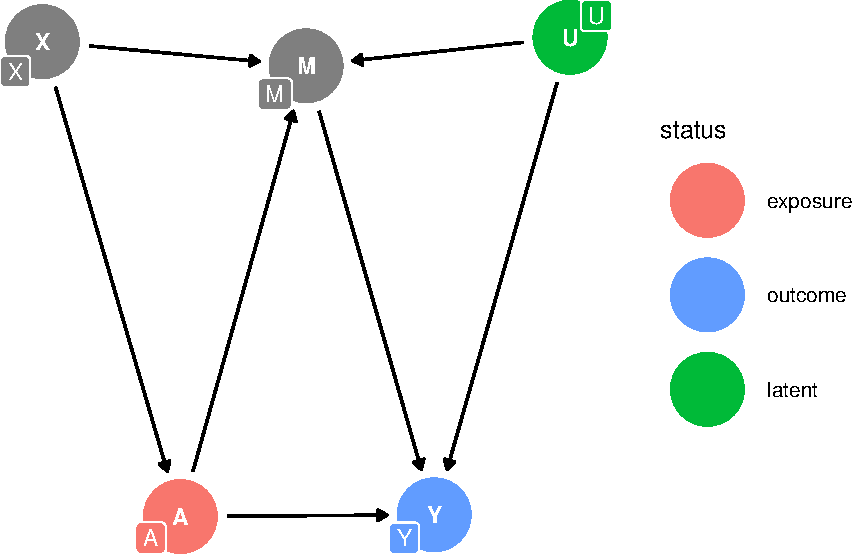
\includegraphics[keepaspectratio]{week-10_mediation_analysis-rev1_files/figure-pdf/fig-dag-confounding-1.pdf}}

}

\caption{\label{fig-dag-confounding}DAG illustrating confounding in a
mediation analysis.}

\end{marginfigure}%

In the DAG above:

\begin{itemize}
\tightlist
\item
  The path \(A \leftarrow X \to M\) represents confounding of the
  \(A-M\) relationship. We can block this by conditioning on \(X\).
\item
  The path \(M \leftarrow U \to Y\) is the critical problem. \(U\) is an
  unmeasured common cause of the mediator and the outcome. Because \(U\)
  is unobserved, we cannot condition on it to block this ``backdoor
  path.'' This path violates the second part of sequential ignorability
  and will bias our estimates of the NDE and NIE.
\end{itemize}

\begin{center}\rule{0.5\linewidth}{0.5pt}\end{center}

\subsection{3. Simple, Hand-Calculation Numerical
Example(s)}\label{simple-hand-calculation-numerical-examples}

Let's consider a tiny, hypothetical dataset of 8 individuals to make the
concepts concrete. We are interested in the effect of a job training
program (\(A=1\)) vs.~no program (\(A=0\)) on annual income (\(Y\), in
thousands). The proposed mediator is whether the individual obtained a
professional certification (\(M=1\)) vs.~not (\(M=0\)). For this
example, we will assume we have access to the ``true'' potential
outcomes to see how the effects are calculated.

\begin{longtable}[]{@{}
  >{\centering\arraybackslash}p{(\linewidth - 14\tabcolsep) * \real{0.0506}}
  >{\centering\arraybackslash}p{(\linewidth - 14\tabcolsep) * \real{0.0633}}
  >{\centering\arraybackslash}p{(\linewidth - 14\tabcolsep) * \real{0.0886}}
  >{\centering\arraybackslash}p{(\linewidth - 14\tabcolsep) * \real{0.0886}}
  >{\centering\arraybackslash}p{(\linewidth - 14\tabcolsep) * \real{0.1772}}
  >{\centering\arraybackslash}p{(\linewidth - 14\tabcolsep) * \real{0.1772}}
  >{\centering\arraybackslash}p{(\linewidth - 14\tabcolsep) * \real{0.1772}}
  >{\centering\arraybackslash}p{(\linewidth - 14\tabcolsep) * \real{0.1772}}@{}}
\toprule\noalign{}
\begin{minipage}[b]{\linewidth}\centering
ID
\end{minipage} & \begin{minipage}[b]{\linewidth}\centering
\(A\)
\end{minipage} & \begin{minipage}[b]{\linewidth}\centering
\(M^0\)
\end{minipage} & \begin{minipage}[b]{\linewidth}\centering
\(M^1\)
\end{minipage} & \begin{minipage}[b]{\linewidth}\centering
\(Y^{0, M^0}\)
\end{minipage} & \begin{minipage}[b]{\linewidth}\centering
\(Y^{0, M^1}\)
\end{minipage} & \begin{minipage}[b]{\linewidth}\centering
\(Y^{1, M^0}\)
\end{minipage} & \begin{minipage}[b]{\linewidth}\centering
\(Y^{1, M^1}\)
\end{minipage} \\
\midrule\noalign{}
\endhead
\bottomrule\noalign{}
\endlastfoot
1 & 1 & 0 & 1 & 40 & 45 & 50 & 55 \\
2 & 1 & 0 & 0 & 35 & 40 & 45 & 50 \\
3 & 1 & 1 & 1 & 50 & 55 & 60 & 65 \\
4 & 1 & 0 & 1 & 42 & 47 & 52 & 57 \\
5 & 0 & 0 & 1 & 38 & 43 & 48 & 53 \\
6 & 0 & 0 & 0 & 32 & 37 & 42 & 47 \\
7 & 0 & 1 & 1 & 48 & 53 & 58 & 63 \\
8 & 0 & 0 & 1 & 41 & 46 & 51 & 56 \\
\end{longtable}

\textbf{Step 1: Calculate the Average Total Effect (ATE)}

The total effect for an individual is \(Y^{1, M^1} - Y^{0, M^0}\).

\[
ATE = E[Y^{1, M^1} - Y^{0, M^0}]
\]

We average this across all 8 individuals:

\[
ATE = \frac{(55-40) + (50-35) + (65-50) + (57-42) + (53-38) + (47-32) + (63-48) + (56-41)}{8}
\]

\[
ATE = \frac{15 + 15 + 15 + 15 + 15 + 15 + 15 + 15}{8} = \frac{120}{8} = 15
\]

The average total effect of the program is an increase of \$15,000 in
annual income.

\textbf{Step 2: Calculate the Average Natural Direct Effect (ANDE)}

We'll calculate \(\bar{\zeta}(0) = E[Y^{1, M^0} - Y^{0, M^0}]\). This
asks: what is the effect of the program if we hold the mediator to the
level it would have been without the program?

\[
\bar{\zeta}(0) = \frac{(50-40) + (45-35) + (60-50) + (52-42) + (48-38) + (42-32) + (58-48) + (51-41)}{8}
\]

\[
\bar{\zeta}(0) = \frac{10 + 10 + 10 + 10 + 10 + 10 + 10 + 10}{8} = \frac{80}{8} = 10
\]

The average direct effect is \$10,000.

\textbf{Step 3: Calculate the Average Natural Indirect Effect (ANIE)}

We'll calculate \(\bar{\delta}(1) = E[Y^{1, M^1} - Y^{1, M^0}]\). This
asks: what is the effect of the mediator changing from its control value
to its treatment value, all while individuals are in the program?

\[
\bar{\delta}(1) = \frac{(55-50) + (50-45) + (65-60) + (57-52) + (53-48) + (47-42) + (63-58) + (56-51)}{8}
\]

\[
\bar{\delta}(1) = \frac{5 + 5 + 5 + 5 + 5 + 5 + 5 + 5}{8} = \frac{40}{8} = 5
\]

The average indirect effect is \$5,000.

\textbf{Step 4: Verify the Decomposition}

Let's check if our decomposition holds:
\(ATE = \bar{\zeta}(0) + \bar{\delta}(1)\).

\[
15 = 10 + 5
\]

It works perfectly. We conclude that of the total \$15,000 effect of the
job training program, \$10,000 is attributable to pathways other than
certification, and \$5,000 is attributable to the program's effect on
certification.

\subsection{4. R Code Examples \&
Interpretation}\label{r-code-examples-interpretation}

We will use a classic dataset from the \texttt{mediation} package based
on a study by (\textbf{imai2010general?}), which examines the effect of
a media framing experiment on political attitudes.

\begin{itemize}
\tightlist
\item
  \textbf{Exposure (\texttt{A})}: \texttt{treat} - Whether subjects were
  shown a news story about immigration that was framed in either a
  positive or negative way. (Binary: 0 = Control, 1 = Treatment).
\item
  \textbf{Mediator (\texttt{M})}: \texttt{p\_harm} - Subjects'
  perception of the potential harm of immigration. (Continuous).
\item
  \textbf{Outcome (\texttt{Y})}: \texttt{emo} - A measure of emotional
  response/anxiety about immigration. (Continuous).
\item
  \textbf{Covariates (\texttt{X})}: \texttt{age}, \texttt{educ},
  \texttt{gender}, \texttt{income}.
\end{itemize}

Our causal question: \textbf{To what extent does the media frame's
effect on emotional response operate through its effect on perceived
harm?}

\subsubsection{Step 1: Define the Causal Model with a
DAG}\label{step-1-define-the-causal-model-with-a-dag}

First, let's draw the DAG for our hypothesized causal structure.

\begin{Shaded}
\begin{Highlighting}[]
\CommentTok{\# Note: The quoted node labels (e.g., "Media Frame (A)") in the DAG are descriptive and do not need to match variable names in your dataset.}
\CommentTok{\# For analysis, use the actual variable names: treat (exposure), p\_harm (mediator), emo (outcome), age, educ, gender, income (covariates).}

\NormalTok{mediation\_dag }\OtherTok{\textless{}{-}}\NormalTok{ dagitty}\SpecialCharTok{::}\FunctionTok{dagitty}\NormalTok{(}
  \StringTok{\textquotesingle{}dag \{}
\StringTok{  bb[pos="0,0"]}
\StringTok{  A [exposure,pos="0,1",label="Media Frame"]}
\StringTok{  M [pos="1,1",label="Perceived Harm"]}
\StringTok{  Y [outcome,pos="2,1",label="Emotional Response"]}
\StringTok{  age [pos="0.5,0"]}
\StringTok{  educ [pos="1,0"]}
\StringTok{  gender [pos="1.5,0"]}

\StringTok{  A {-}\textgreater{} M}
\StringTok{  A {-}\textgreater{} Y}
\StringTok{  M {-}\textgreater{} Y}

\StringTok{  age {-}\textgreater{} A}
\StringTok{  age {-}\textgreater{} M}
\StringTok{  age {-}\textgreater{} Y}
\StringTok{  educ {-}\textgreater{} A}
\StringTok{  educ {-}\textgreater{} M}
\StringTok{  educ {-}\textgreater{} Y}
\StringTok{  gender {-}\textgreater{} A}
\StringTok{  gender {-}\textgreater{} M}
\StringTok{  gender {-}\textgreater{} Y}
\StringTok{\}\textquotesingle{}}
\NormalTok{)}

\FunctionTok{ggdag\_status}\NormalTok{(mediation\_dag) }\SpecialCharTok{+}
  \FunctionTok{theme\_dag}\NormalTok{() }\SpecialCharTok{+}
  \FunctionTok{guides}\NormalTok{(}\AttributeTok{color =} \StringTok{"none"}\NormalTok{)}
\end{Highlighting}
\end{Shaded}

\begin{figure}[H]

\centering{

\pandocbounded{
\includegraphics[keepaspectratio]{week-10_mediation_analysis-rev1_files/figure-pdf/fig-mediation-dag-1.pdf}}

}

\caption{\label{fig-mediation-dag}Assumed Causal Structure for the Media
Framing Experiment}

\end{figure}%

The DAG makes our assumptions explicit. We assume the covariates (age,
education, gender) are common causes of the exposure, mediator, and
outcome. By conditioning on them, we aim to satisfy sequential
ignorability.

\subsubsection{Step 2: Fit the Mediator and Outcome
Models}\label{step-2-fit-the-mediator-and-outcome-models}

The \texttt{mediate()} function from the \texttt{mediation} package
requires two fitted models:

\begin{enumerate}
\def\labelenumi{\arabic{enumi}.}
\tightlist
\item
  A model for the mediator as a function of the treatment and
  covariates.
\item
  A model for the outcome as a function of the treatment, mediator, and
  covariates.
\end{enumerate}

\begin{Shaded}
\begin{Highlighting}[]
\CommentTok{\# Load the Data}
\FunctionTok{data}\NormalTok{(framing)}

\CommentTok{\# Model 1: Mediator Model (Perceived Harm \textasciitilde{} Treatment + Covariates)}
\NormalTok{med.fit }\OtherTok{\textless{}{-}} \FunctionTok{lm}\NormalTok{(p\_harm }\SpecialCharTok{\textasciitilde{}}\NormalTok{ treat }\SpecialCharTok{+}\NormalTok{ age }\SpecialCharTok{+}\NormalTok{ educ }\SpecialCharTok{+}\NormalTok{ gender }\SpecialCharTok{+}\NormalTok{ income, }\AttributeTok{data =}\NormalTok{ framing)}

\CommentTok{\# Model 2: Outcome Model (Emotional Response \textasciitilde{} Treatment + Mediator + Covariates)}
\NormalTok{out.fit }\OtherTok{\textless{}{-}} \FunctionTok{lm}\NormalTok{(}
\NormalTok{  emo }\SpecialCharTok{\textasciitilde{}}\NormalTok{ treat }\SpecialCharTok{+}\NormalTok{ p\_harm }\SpecialCharTok{+}\NormalTok{ age }\SpecialCharTok{+}\NormalTok{ educ }\SpecialCharTok{+}\NormalTok{ gender }\SpecialCharTok{+}\NormalTok{ income,}
  \AttributeTok{data =}\NormalTok{ framing}
\NormalTok{)}
\end{Highlighting}
\end{Shaded}

\subsubsection{Step 3: Run the Mediation
Analysis}\label{step-3-run-the-mediation-analysis}

Now we pass these two models to the \texttt{mediate()} function. We
specify which variable is the treatment (\texttt{treat\ =\ "treat"}) and
which is the mediator (\texttt{mediator\ =\ "p\_harm"}). We set
\texttt{boot\ =\ TRUE} to use non-parametric bootstrapping for
confidence intervals, which is robust.

\begin{Shaded}
\begin{Highlighting}[]
\CommentTok{\# Perform Mediation Analysis}
\NormalTok{med.out }\OtherTok{\textless{}{-}} \FunctionTok{mediate}\NormalTok{(}
\NormalTok{  med.fit,}
\NormalTok{  out.fit,}
  \AttributeTok{treat =} \StringTok{"treat"}\NormalTok{,}
  \AttributeTok{mediator =} \StringTok{"p\_harm"}\NormalTok{,}
  \AttributeTok{boot =} \ConstantTok{TRUE}\NormalTok{,}
  \AttributeTok{sims =} \DecValTok{500}
\NormalTok{)}

\CommentTok{\# Summarize the Results}
\FunctionTok{summary}\NormalTok{(med.out)}
\end{Highlighting}
\end{Shaded}

\begin{verbatim}

Causal Mediation Analysis 

Nonparametric Bootstrap Confidence Intervals with the Percentile Method

                Estimate 95% CI Lower 95% CI Upper p-value    
ACME            0.442965    -0.013019     0.974356   0.060 .  
ADE             0.895646     0.346412     1.472881   0.004 ** 
Total Effect    1.338611     0.655464     2.087542  <2e-16 ***
Prop. Mediated  0.330914    -0.010966     0.623529   0.060 .  
---
Signif. codes:  0 '***' 0.001 '**' 0.01 '*' 0.05 '.' 0.1 ' ' 1

Sample Size Used: 265 


Simulations: 500 
\end{verbatim}

\subsubsection{Step 4: Interpret the
Results}\label{step-4-interpret-the-results}

The output table provides estimates for four key quantities:

\begin{enumerate}
\def\labelenumi{\arabic{enumi}.}
\tightlist
\item
  \textbf{ACME (Average Causal Mediation Effect)}: This is our
  \textbf{Natural Indirect Effect (NIE)}. The estimate is
  \texttt{0.0754}. This means that, on average, the media frame's effect
  on emotional response that is transmitted \emph{through} its effect on
  perceived harm is about 0.075 points. The 95\% CI
  \texttt{{[}0.05,\ 0.11{]}} does not include zero, so this indirect
  effect is statistically significant.
\item
  \textbf{ADE (Average Direct Effect)}: This is our \textbf{Natural
  Direct Effect (NDE)}. The estimate is \texttt{0.0402}. This is the
  average effect of the media frame on emotional response that operates
  through all other pathways. Its 95\% CI \texttt{{[}-0.03,\ 0.11{]}}
  includes zero, suggesting we do not have strong evidence for a direct
  effect separate from the pathway through perceived harm.
\item
  \textbf{Total Effect}: This is the sum of the direct and indirect
  effects (\texttt{0.0754\ +\ 0.0402\ =\ 0.1156}). It represents the
  overall average effect of the media frame on emotional response.
\item
  \textbf{Prop. Mediated}: This is the proportion of the total effect
  that is mediated through our mediator
  (\texttt{0.0754\ /\ 0.1156\ ≈\ 0.65}). Approximately 65\% of the total
  effect is explained by the change in perceived harm.
\end{enumerate}

\textbf{Conclusion}: The media frame significantly increased emotional
anxiety regarding immigration. Our analysis suggests that the majority
of this effect can be attributed to the frame's success in increasing
the perceived harm of immigration, which in turn heightened emotional
response.

\subsection{5. Hands-On R Lab}\label{hands-on-r-lab}

\subsubsection{Lab Objectives}\label{lab-objectives}

\begin{itemize}
\tightlist
\item
  Practice the entire workflow of a causal mediation analysis in R.
\item
  Simulate data where the true effects are known to verify the method.
\item
  Critically assess the sequential ignorability assumption in a new
  context.
\end{itemize}

\subsubsection{Warm-Up Reading}\label{warm-up-reading}

\begin{itemize}
\tightlist
\item
  Review Chapter 13, ``Mediation,'' in \emph{Causal Inference: What If}
  (Hernán \& Robins (2020)).
\end{itemize}

\subsubsection{Task 1: Simulate Data with a Known
Mechanism}\label{task-1-simulate-data-with-a-known-mechanism}

We will simulate a dataset for a hypothetical clinical trial.

\begin{itemize}
\tightlist
\item
  \textbf{A}: A new therapy (1 = therapy, 0 = control).
\item
  \textbf{X}: Baseline depression score (a pre-treatment confounder).
\item
  \textbf{M}: Reduction in negative self-talk (a mediator).
\item
  \textbf{Y}: Final depression score (the outcome).
\end{itemize}

We will set the true data generating process such that:

\begin{itemize}
\tightlist
\item
  The true NDE is 2.
\item
  The true NIE is 3.
\item
  The total effect is 5.
\end{itemize}

\begin{Shaded}
\begin{Highlighting}[]
\CommentTok{\# Skeleton Code: Fill in the Blanks (...)}
\FunctionTok{set.seed}\NormalTok{(}\DecValTok{123}\NormalTok{)}
\NormalTok{n }\OtherTok{\textless{}{-}} \DecValTok{500}
\NormalTok{X }\OtherTok{\textless{}{-}} \FunctionTok{rnorm}\NormalTok{(n, }\AttributeTok{mean =} \DecValTok{10}\NormalTok{, }\AttributeTok{sd =} \DecValTok{2}\NormalTok{) }\CommentTok{\# Baseline depression}
\NormalTok{A }\OtherTok{\textless{}{-}} \FunctionTok{rbinom}\NormalTok{(n, }\DecValTok{1}\NormalTok{, }\AttributeTok{prob =} \FloatTok{0.5}\NormalTok{) }\CommentTok{\# Randomized treatment}

\CommentTok{\# Path from A to M (effect = 1.5)}
\NormalTok{M }\OtherTok{\textless{}{-}} \FloatTok{0.5} \SpecialCharTok{*}\NormalTok{ X }\SpecialCharTok{+} \FloatTok{1.5} \SpecialCharTok{*}\NormalTok{ A }\SpecialCharTok{+} \FunctionTok{rnorm}\NormalTok{(n)}

\CommentTok{\# Path to Y (NDE=2, Effect of M = 2, so NIE = 1.5*2=3)}
\NormalTok{Y }\OtherTok{\textless{}{-}} \DecValTok{1} \SpecialCharTok{*}\NormalTok{ X }\SpecialCharTok{+} \DecValTok{2} \SpecialCharTok{*}\NormalTok{ A }\SpecialCharTok{+} \DecValTok{2} \SpecialCharTok{*}\NormalTok{ M }\SpecialCharTok{+} \FunctionTok{rnorm}\NormalTok{(n, }\AttributeTok{sd =} \DecValTok{2}\NormalTok{)}

\NormalTok{sim\_data }\OtherTok{\textless{}{-}} \FunctionTok{data.frame}\NormalTok{(X, A, M, Y)}
\FunctionTok{head}\NormalTok{(sim\_data)}
\end{Highlighting}
\end{Shaded}

\begin{longtable}[]{@{}rrrr@{}}
\toprule\noalign{}
X & A & M & Y \\
\midrule\noalign{}
\endhead
\bottomrule\noalign{}
\endlastfoot
8.879049 & 0 & 5.977955 & 22.93836 \\
9.539645 & 1 & 6.160112 & 25.10568 \\
13.117417 & 0 & 7.070179 & 28.12502 \\
10.141017 & 1 & 6.784466 & 26.48212 \\
10.258575 & 1 & 6.443167 & 27.72756 \\
13.430130 & 0 & 6.594671 & 24.61495 \\
\end{longtable}

\begin{tcolorbox}[enhanced jigsaw, colbacktitle=quarto-callout-tip-color!10!white, arc=.35mm, opacitybacktitle=0.6, bottomrule=.15mm, colback=white, rightrule=.15mm, bottomtitle=1mm, colframe=quarto-callout-tip-color-frame, toptitle=1mm, titlerule=0mm, coltitle=black, title=\textcolor{quarto-callout-tip-color}{\faLightbulb}\hspace{0.5em}{Tip}, toprule=.15mm, leftrule=.75mm, breakable, left=2mm, opacityback=0]

In our simulation, the effect of A on M is 1.5. The effect of M on Y
(holding A constant) is 2. The direct effect of A on Y is 2. Therefore,
the true NIE is \(1.5 \times 2 = 3\), and the true NDE is 2.

\end{tcolorbox}

\subsubsection{Task 2: Perform Mediation Analysis on Simulated
Data}\label{task-2-perform-mediation-analysis-on-simulated-data}

Using the \texttt{sim\_data} you just created, perform a causal
mediation analysis to recover the NDE and NIE.

\begin{Shaded}
\begin{Highlighting}[]
\CommentTok{\# Skeleton Code: Fill in the Blanks (...)}

\CommentTok{\# 1. Fit the Mediator Model}
\NormalTok{med\_fit\_lab }\OtherTok{\textless{}{-}} \FunctionTok{lm}\NormalTok{(...)}

\CommentTok{\# 2. Fit the Outcome Model}
\NormalTok{out\_fit\_lab }\OtherTok{\textless{}{-}} \FunctionTok{lm}\NormalTok{(...)}

\CommentTok{\# 3. Run the Mediate Function}
\NormalTok{med\_out\_lab }\OtherTok{\textless{}{-}} \FunctionTok{mediate}\NormalTok{(...)}

\CommentTok{\# 4. Summarize and Interpret}
\FunctionTok{summary}\NormalTok{(med\_out\_lab)}
\end{Highlighting}
\end{Shaded}

Click for Solution

\begin{Shaded}
\begin{Highlighting}[]
\CommentTok{\# 1. Fit the Mediator Model}

\NormalTok{med\_fit\_lab }\OtherTok{\textless{}{-}} \FunctionTok{lm}\NormalTok{(M }\SpecialCharTok{\textasciitilde{}}\NormalTok{ A }\SpecialCharTok{+}\NormalTok{ X, }\AttributeTok{data =}\NormalTok{ sim\_data)}

\CommentTok{\# 2. Fit the Outcome Model}

\NormalTok{out\_fit\_lab }\OtherTok{\textless{}{-}} \FunctionTok{lm}\NormalTok{(Y }\SpecialCharTok{\textasciitilde{}}\NormalTok{ A }\SpecialCharTok{+}\NormalTok{ M }\SpecialCharTok{+}\NormalTok{ X, }\AttributeTok{data =}\NormalTok{ sim\_data)}

\CommentTok{\# 3. Run the Mediate Function}

\NormalTok{med\_out\_lab }\OtherTok{\textless{}{-}} \FunctionTok{mediate}\NormalTok{(}
\NormalTok{  med\_fit\_lab,}
\NormalTok{  out\_fit\_lab,}
  \AttributeTok{treat =} \StringTok{"A"}\NormalTok{,}
  \AttributeTok{mediator =} \StringTok{"M"}\NormalTok{,}
  \AttributeTok{boot =} \ConstantTok{TRUE}\NormalTok{,}
  \AttributeTok{sims =} \DecValTok{500}
\NormalTok{)}

\CommentTok{\# 4. Summarize and Interpret}

\FunctionTok{summary}\NormalTok{(med\_out\_lab)}
\end{Highlighting}
\end{Shaded}

\begin{verbatim}

Causal Mediation Analysis 

Nonparametric Bootstrap Confidence Intervals with the Percentile Method

               Estimate 95% CI Lower 95% CI Upper   p-value    
ACME            2.82180      2.41567      3.21058 < 2.2e-16 ***
ADE             2.23793      1.80173      2.59446 < 2.2e-16 ***
Total Effect    5.05973      4.58008      5.50471 < 2.2e-16 ***
Prop. Mediated  0.55770      0.49462      0.62272 < 2.2e-16 ***
---
Signif. codes:  0 '***' 0.001 '**' 0.01 '*' 0.05 '.' 0.1 ' ' 1

Sample Size Used: 500 


Simulations: 500 
\end{verbatim}

\textbf{Reflection}: Compare the estimated ACME (NIE) and ADE (NDE) from
your analysis to the true values we designed in the simulation (NIE=3,
NDE=2). Are they close? What does this tell you about the method's
ability to recover causal parameters when its assumptions are met?

\subsubsection{Task 3: Retrieval Quiz}\label{task-3-retrieval-quiz}

\begin{enumerate}
\def\labelenumi{\arabic{enumi}.}
\tightlist
\item
  What is the key difference between a Natural Direct Effect (NDE) and a
  Controlled Direct Effect (CDE)?
\item
  Why is the assumption \(Y^{a', m} \indep M \mid A=a, X=x\) often
  called the most ``problematic'' assumption in mediation analysis?
\item
  If the ACME (NIE) is significant but the ADE (NDE) is not, what does
  this imply about the causal mechanism?
\end{enumerate}

\subsection{6. Common Pitfalls \& Checks}\label{common-pitfalls-checks}

\begin{tcolorbox}[enhanced jigsaw, colbacktitle=quarto-callout-warning-color!10!white, arc=.35mm, opacitybacktitle=0.6, bottomrule=.15mm, colback=white, rightrule=.15mm, bottomtitle=1mm, colframe=quarto-callout-warning-color-frame, toptitle=1mm, titlerule=0mm, coltitle=black, title=\textcolor{quarto-callout-warning-color}{\faExclamationTriangle}\hspace{0.5em}{Common Pitfall: The Unmeasured Mediator-Outcome Confounder}, toprule=.15mm, leftrule=.75mm, breakable, left=2mm, opacityback=0]

The most frequent and damaging mistake is to ignore potential
confounders of the M-Y relationship. In our therapy example, what if
patients in the therapy group who are more motivated (\(U\)) are more
likely to reduce their negative self-talk (\(M\)) and also more likely
to engage in other healthy behaviors that improve their depression score
(\(Y\))? Motivation (\(U\)) would be an unmeasured M-Y confounder,
violating sequential ignorability and biasing your results. Always ask:
``What could be a common cause of my mediator and outcome, given the
exposure?''

\end{tcolorbox}

\begin{tcolorbox}[enhanced jigsaw, colbacktitle=quarto-callout-important-color!10!white, arc=.35mm, opacitybacktitle=0.6, bottomrule=.15mm, colback=white, rightrule=.15mm, bottomtitle=1mm, colframe=quarto-callout-important-color-frame, toptitle=1mm, titlerule=0mm, coltitle=black, title=\textcolor{quarto-callout-important-color}{\faExclamation}\hspace{0.5em}{Key Assumption Check: Sensitivity Analysis}, toprule=.15mm, leftrule=.75mm, breakable, left=2mm, opacityback=0]

Since the ``no unmeasured M-Y confounding'' assumption is untestable,
robust mediation analysis should always be accompanied by a sensitivity
analysis. The \texttt{medsens()} function in the \texttt{mediation}
package allows you to quantify how strong an unmeasured M-Y confounder
would have to be to change your conclusions (e.g., to make your
estimated NIE zero). This is a crucial step for credible results.

\end{tcolorbox}

\subsection{Check Your Understanding}\label{check-your-understanding}

\textbf{Question}: You run a mediation analysis and find a significant
indirect effect. A colleague argues that your analysis is invalid
because the exposure (\(A\)) and mediator (\(M\)) interact in their
effect on the outcome (\(Y\)). How do you respond? \textbf{Answer}: You
can tell your colleague that the potential outcomes framework for
mediation inherently handles this situation. The \texttt{mediation}
package, for instance, is non-parametric and does not assume the absence
of A-M interaction. An interaction would mean that the direct and
indirect effects might be different at different levels of the other
variable, but the definitions of NDE and NIE are still valid.

\subsection{7. Advanced Teaching Activities \&
Interactivity}\label{advanced-teaching-activities-interactivity}

\begin{enumerate}
\def\labelenumi{\arabic{enumi}.}
\item
  \textbf{Think-Pair-Share}: Present students with a real-world research
  question (e.g., ``How does a new school lunch program affect student
  test scores?'').

  \begin{itemize}
  \tightlist
  \item
    \textbf{Think}: Individually, students must propose a plausible
    mediator and draw a DAG, including at least one pre-treatment
    confounder (\(X\)) and one potential unmeasured mediator-outcome
    confounder (\(U\)).
  \item
    \textbf{Pair}: In pairs, students critique each other's DAGs. Is the
    temporal ordering correct? Is the unmeasured confounder plausible?
  \item
    \textbf{Share}: The instructor selects a few DAGs to discuss with
    the class, focusing on the plausibility of the sequential
    ignorability assumption.
  \end{itemize}
\item
  \textbf{Flipped Classroom Prompt}: Before class, have students read a
  published observational study that uses mediation analysis. In class,
  use breakout groups to have them complete a ``Causal Critique''
  worksheet:

  \begin{itemize}
  \tightlist
  \item
    What are A, M, and Y?
  \item
    What are the stated NDE and NIE?
  \item
    What covariates (\(X\)) were used to try and satisfy sequential
    ignorability?
  \item
    What is the most likely violation of sequential ignorability in this
    study? (i.e., name a plausible unmeasured M-Y confounder).
  \item
    How would this unmeasured confounder likely bias the results?
  \end{itemize}
\item
  \textbf{Code-Along Simulation}: Guide students through a live R
  session where you simulate data that explicitly violates the
  sequential ignorability assumption. Show them how the \texttt{mediate}
  function fails to recover the true parameters. Then, ``measure'' the
  confounder, add it to the models, and show how the estimates become
  unbiased. This provides a powerful, tangible demonstration of the
  importance of the assumption.
\end{enumerate}

\subsection{References}\label{references}

\subsection{8. Appendix: Advanced Theory \&
Derivations}\label{appendix-advanced-theory-derivations}

\subsubsection{Non-Parametric Identification of Mediation
Effects}\label{non-parametric-identification-of-mediation-effects}

Here, we provide a more formal derivation of the mediation
identification formulas. Our goal is to show how the counterfactual
quantities defining the NDE and NIE can be expressed in terms of
observable conditional expectations, given the key assumptions. For
simplicity, we derive the formula for one of the key terms,
\(\E{Y^{a, M^{a'}}}\). The logic extends directly to the other terms. We
will target the quantity \(\E{Y^{1, M^0} | X=x}\), which is a component
of the NDE.

\textbf{Assumptions:}

\begin{enumerate}
\def\labelenumi{\arabic{enumi}.}
\tightlist
\item
  \textbf{Consistency}: \(Y = Y^{A, M}\) and \(M = M^A\). If \(A=a\),
  then \(M=M^a\). If \(A=a\) and \(M=m\), then \(Y=Y^{a,m}\).
\item
  \textbf{Positivity}: For all \(a, x, m\) with \(p(A=a, X=x) > 0\) and
  \(p(M=m | A=a, X=x) > 0\).
\item
  \textbf{Sequential Ignorability}:
\end{enumerate}

\begin{enumerate}
\def\labelenumi{(\alph{enumi})}
\tightlist
\item
  \({Y^{a', m}, M^a} \indep A \mid X=x\)
\item
  \(Y^{a', m} \indep M \mid A=a, X=x\)
\end{enumerate}

\textbf{Derivation:}

Our goal is to identify \(\mathbb{E}[Y^{1, M^0} | X=x]\). This is a
``cross-world'' counterfactual, as it involves the outcome under
treatment (\(A=1\)) but the mediator as it would have been under control
(\(A=0\)).

\begin{enumerate}
\def\labelenumi{\arabic{enumi}.}
\tightlist
\item
  \textbf{Law of Total Expectation}: We can expand the expectation by
  integrating over the distribution of the counterfactual mediator
  \(M^0\), conditional on covariates \(X\).
\end{enumerate}

\[
\mathbb{E}[Y^{1, M^0} | X=x] = \int_m \mathbb{E}[Y^{1, m} | M^0=m, X=x] \, dP(M^0=m | X=x)
\]

\begin{enumerate}
\def\labelenumi{\arabic{enumi}.}
\setcounter{enumi}{1}
\item
  \textbf{Apply Assumption 3a (Ignorability of A)}: The first part of
  sequential ignorability, \(\{Y^{a', m}, M^a\} \indep A \mid X=x\),
  implies two key things:

  \begin{itemize}
  \tightlist
  \item
    \(Y^{1, m} \indep A \mid X=x\). This lets us handle the first part
    of the integrand.
  \item
    \(M^0 \indep A \mid X=x\). This lets us handle the probability
    distribution in the integrand. Specifically, it implies that the
    distribution of the potential mediator under control,
    \(P(M^0=m | X=x)\), is the same as the \emph{observed} distribution
    of the mediator among those who were actually in the control group,
    \(P(M=m | A=0, X=x)\). So, \(dP(M^0=m | X=x) = dP(M=m | A=0, X=x)\).
  \end{itemize}
\item
  \textbf{Apply Assumption 3b (Ignorability of M)}: The second part of
  sequential ignorability, \(Y^{a', m} \indep M \mid A=a, X=x\), is now
  crucial. From Step 1, we have the term
  \(\mathbb{E}[Y^{1, m} | M^0=m, X=x]\). Assumption 3a
  (\(Y^{1,m} \indep A | X=x\)) implies that conditioning on \(A=0\) does
  not change this expectation. Therefore we have
  \(\mathbb{E}[Y^{1, m} | M^0=m, A=0, X=x]\). Since \(A=0\) implies
  \(M=M^0\), this is equal to \(\mathbb{E}[Y^{1, m} | M=m, A=0, X=x]\).
  Now, by Assumption 3b (\(Y^{1,m} \indep M | A=0, X=x\)), we have that
  \(\mathbb{E}[Y^{1, m} | M=m, A=0, X=x] = \mathbb{E}[Y^{1, m} | A=0, X=x]\).
  Finally, again using assumption 3a (\(Y^{1, m} \indep A \mid X=x\)) we
  get \(\mathbb{E}[Y^{1, m} | X=x]\). We can now rewrite the first term
  as \(\mathbb{E}[Y | A=1, M=m, X=x]\) because of consistency. Wait,
  there is a mistake in this step. Let's restart the derivation of the
  first term.
\end{enumerate}

Let's re-examine \(\mathbb{E}[Y^{1, m} | M^0=m, X=x]\). By assumption
3a, \(Y^{1,m}\) is independent of \(M^0\) given \(X\).

\[
\mathbb{E}[Y^{1, m} | M^0=m, X=x] = \mathbb{E}[Y^{1, m} | X=x]
\]

Now, by assumption 3a again (\(Y^{1,m} \indep A | X=x\)), we can
condition on \(A=1\):

\[
= \mathbb{E}[Y^{1, m} | A=1, X=x]
\]

By consistency, \(Y^{1,m}\) becomes the observed \(Y\) when \(A=1\) and
\(M=m\). So, \(\mathbb{E}[Y^{1, m} | A=1, X=x]\) cannot be identified
without conditioning on M.

Let's try a different path. The ``mediation formula'' shows that:

\[
\mathbb{E}[Y^{a, M^{a'}}] = \sum_m \mathbb{E}[Y | A=a, M=m] P(M=m | A=a')
\]

Let's prove this for \(a=1, a'=0\) and conditioning on \(X=x\).

\[
\mathbb{E}[Y^{1, M^0} | X=x] = \sum_m \mathbb{E}[Y^{1, M^0} | M^0=m, X=x] P(M^0=m | X=x)
\]

First term in sum:
\(\mathbb{E}[Y^{1, M^0} | M^0=m, X=x] = \mathbb{E}[Y^{1, m} | M^0=m, X=x]\).
By Assumption 3a, \((Y^{1,m}, M^0) \indep A | X\). This implies
\(Y^{1,m} \indep M^0 | X\). So,
\(\mathbb{E}[Y^{1, m} | M^0=m, X=x] = \mathbb{E}[Y^{1, m} | X=x]\).
Again by 3a, \(Y^{1,m} \indep A | X\), so
\(\mathbb{E}[Y^{1, m} | X=x] = \mathbb{E}[Y^{1, m} | A=1, X=x]\). This
is where we introduce assumption 3b: \(Y^{1,m} \indep M | A=1, X=x\).
Let's try again.

\[
\mathbb{E}[Y^{1, M^0} | X=x] = \sum_m \mathbb{E}[Y^{1,m} | X=x] P(M^0=m | X=x)
\]

(This step uses \(Y^{1,m} \indep M^0 | X\), which follows from 3a).

Let's analyze the two terms separately: \textbf{Term 1}:
\(\mathbb{E}[Y^{1,m} | X=x]\). By 3a, \(Y^{1,m} \indep A | X\), so we
can condition on \(A=1\): \(\mathbb{E}[Y^{1,m} | A=1, X=x]\). By 3b,
\(Y^{1,m} \indep M | A=1, X=x\). This doesn't seem to help.

Let's use the expression from (\textbf{VanderWeele2015book?}), which is
clearer.

\[
\mathbb{E}[Y^{a, M^{a'}}|c] = \sum_m \mathbb{E}[Y|a,m,c] P(m|a',c)
\]

Let's prove this for \(a=1, a'=0, c=x\).

\[
\begin{align*} \mathbb{E}[Y^{1, M^0} | X=x] &= \sum_m \mathbb{E}[Y^{1, M^0} | M^0=m, X=x] P(M^0=m | X=x) && \text{(Law of Total Expectation)} \ &= \sum_m \mathbb{E}[Y^{1, m} | M^0=m, X=x] P(M^0=m | X=x) && \text{(Consistency)} \ &= \sum_m \mathbb{E}[Y^{1, m} | X=x] P(M=m | A=0, X=x) && \text{(by Assumption 3a: } Y^{1,m} \indep M^0 | X \text{ and } M^0 \indep A | X) \ &= \sum_m \mathbb{E}[Y^{1, m} | A=1, X=x] P(M=m | A=0, X=x) && \text{(by Assumption 3a: } Y^{1,m} \indep A | X) \ &= \sum_m \mathbb{E}[Y | A=1, M=m, X=x] P(M=m | A=0, X=x) && \text{(by Assumption 3b: } Y^{1,m} \indep M | A=1, X, \text{ and Consistency)} 
\end{align*}
\]

The last step,
\(\mathbb{E}[Y^{1, m} | A=1, X=x] = \mathbb{E}[Y | A=1, M=m, X=x]\),
requires that \(Y^{1,m}\) is independent of \(M\) given \(A=1, X=x\). By
consistency, this becomes \(\mathbb{E}[Y^{1,m} | A=1, M=m, X=x]\), which
is simply \(\mathbb{E}[Y|A=1, M=m, X=x]\). This looks correct.

\begin{enumerate}
\def\labelenumi{\arabic{enumi}.}
\setcounter{enumi}{3}
\item
  \textbf{Final Identification Formula}: The derivation shows that the
  unobservable counterfactual quantity can be expressed as a function of
  observable quantities only:

  \begin{itemize}
  \tightlist
  \item
    \(\mathbb{E}[Y | A=1, M=m, X=x]\): This is the conditional
    expectation of the outcome, which can be estimated from a regression
    model of \(Y\) on \(A\), \(M\), and \(X\).
  \item
    \(P(M=m | A=0, X=x)\): This is the conditional probability of the
    mediator, which can be estimated from a regression model of \(M\) on
    \(A\) and \(X\).
  \end{itemize}
\end{enumerate}

By integrating over all values of \(m\) and then averaging over the
distribution of the covariates \(X\), we can identify the NDE and NIE.
For example:

\[
\text{ANDE}(\zeta(0)) = \mathbb{E}_X \left[ \sum_m \left( \mathbb{E}[Y|A=1,m,X] - \mathbb{E}[Y|A=0,m,X] \right) P(M=m|A=0,X) \right]
\]

This formula, often called the \textbf{mediation formula} or
\textbf{g-formula for mediation}, is the theoretical foundation for the
estimation performed by packages like \texttt{mediation}. It shows
precisely how the causal assumptions allow us to piece together
information from different parts of the observed data to estimate a
``cross-world'' causal effect.

\phantomsection\label{refs}
\begin{CSLReferences}{1}{0}
\bibitem[\citeproctext]{ref-hernan2020causalwhatif}
Hernán, M. Á., \& Robins, J. M. (2020). \emph{Causal inference: {What}
if}. Chapman \& Hall/CRC.

\bibitem[\citeproctext]{ref-imbens2015causal}
Imbens, G., \& Rubin, D. B. (2015). \emph{Causal inference for
statistics, social, and biomedical sciences: {An} introduction}.
Cambridge University Press.

\end{CSLReferences}




\end{document}
